% Semi-automatisation du modèle

\section{Automatisation et semi-automatisation}
La mission de l'Inria sur le projet EHRI est de proposer un soutien technique, que les éditeur$\cdot$ice$\cdot$s sont libres d'utiliser ou non. Si certaines tâches peuvent être automatisées, à l'aide de \textit{scripts} Python par exemple, leur utilisation n'est pas forcément à la portée de tout le monde et les éditeur$\cdot$ice$\cdot$s pourraient préférer une solution plus accessible.  

La créatrice de l'application DiScholEd, Floriane Chiffoleau, a rédigé une série de \textit{scripts} d'automatisation\footnote{Voir le dépôt GitHub du projet DAHN~: \texttt{\href{https://github.com/FloChiff/DAHNProject}{https://github.com/FloChiff/DAHNProject}}.} de plusieurs étapes de la chaîne éditoriale, notamment concernant l'encodage des métadonnées et la gestion des entités nommées. L'adaptation de ces \textit{scripts} aux collections de l'EHRI fait partie des prochaines étapes du travail sur le projet.  

Il n'est actuellement pas envisageable d'automatiser tout ou partie de la chaîne éditoriale des éditions EHRI. C'est pourquoi nous avons opté pour une semi-automatisation du processus d'encodage en proposant aux éditeur$\cdot$ice$\cdot$s des \textit{templates} (\enquote{modèles\footnote{Nous utiliserons le terme anglais \enquote{\textit{template}} afin d'établir une distinction avec la notion de \enquote{modèle d'encodage}, qui fait référence à l'ODD et aux règles mises en place.}}) pour l'encodage de certaines parties des fichiers.



\section{Création des \textit{templates} d'encodage}
Nous avons créé deux sortes de \textit{templates} d'encodage. Le premier, et le plus conséquent, concerne l'encodage des métadonnées (Annexe \ref{Metadonnees})~; le second concerne les entrées des index. Il existe trois index aux éditions EHRI~: un index de lieux, un index de personnes et un index des organisations. Nous avons créé un quatrième \textit{template} pour un \enquote{index de termes}. Actuellement, des renvois sont faits vers le vocabulaire contrôlé disponible sur le portail de l'EHRI\footnote{Vocabulaire sur le portail de l'EHRI~: \texttt{\href{https://portal.ehri-project.eu/vocabularies}{https://portal.ehri-project.eu/vocabularies}}.}.  

L'idée derrière la création de ces \textit{templates} est de permettre aux éditeur$\cdot$ice$\cdot$s de gagner du temps en leur proposant une structure à compléter. Cela permet de s'assurer que le plus de champs seront renseignés, et d'éviter des confusions entre différents éléments.  

\begin{figure}[h]
    \centering
    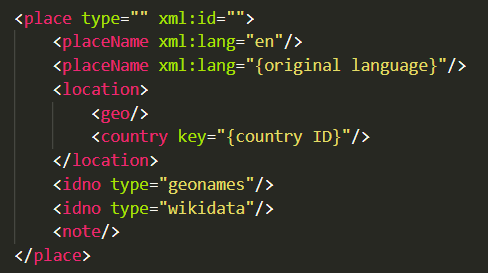
\includegraphics[width=0.7\linewidth]{2-MAIN/images/index.png}
    \caption{\textit{Template} d'une entrée dans l'index de lieux}
    \label{fig:index}
\end{figure}

La Figure \ref{fig:index} représente le \textit{template} d'entrée dans l'index de lieux. Il est bien sûr possible d'ajouter des éléments \texttt{<placeName>} pour chaque langue si le nom du lieu a été traduit, tout comme il est possible de supprimer l'élément \texttt{<placeName xml:lang="en">} si le nom du lieu est typique de sa langue originale et n'a jamais été traduit. L'objectif n'est pas de proposer une traduction, mais de la renseigner, si elle existe, pour faciliter la recherche d'information. Nous estimons qu'il est important d'établir un lien entre les index des éditions et les bases de données publiques largement utilisées comme Geonames\footnote{Geonames~: \texttt{\href{https://www.geonames.org/}{https://www.geonames.org/}}.} et Wikidata\footnote{Wikidata~: \texttt{\href{https://www.wikidata.org/wiki/Wikidata:Main_Page}{https://www.wikidata.org/}}.}, lorsque cela est possible.